There are two major sections into which the design solution can be divided. These two section are data and implementation. 

\subsection{Data}

The data section of our design solution includes anything relevant to data, including collecting, storing, and accessing the data.
\subsubsection{Collecting Data}
Initially we had two candidates for the primary source of obtaining all nba player and team related statistics. These two sources were: 
\begin{itemize}
\item stats.nba.com
\item basketball-reference.com
\end{itemize}
Both sources contained similar amounts of information on player matches, player season averages, teams, matches, with basket-ball reference being slightly more detailed in aspects such as player season averages and player matches. While both sources were credible, we decided to pursue stats.nba.com as the primary source as we felt the official statistics platform of the NBA would have more reliable data compared to one that is not affiliated.

The collection of data from stats.nba.com is done by finding a webpage with pertinent data, scraping that data using Python, and storing it in a MySQL database. We automated the process of scraping the data by writing python scripts that iterate through all web pages of a specified type and searching through HTML tags to retrieve the desired data. This usually entails locating and HTML table, iterating through it's rows and columns, and retrieving stats for points, assists, rebounds, etc. The two fundamental tools used in the scraping process were the python libraries:
\begin{itemize}
\item BeautifulSoup4
\item Selenium
\end{itemize}

BeautifulSoup allows for objectification of HTML tags on a web page such that can be accessed  through Python and Selenium automates the usage of a chosen browser. While, in most cases, BeautifulSoup alone would be enough to simply access the HTML elements of a given web page, stats.nba.com generates all of the data that we need through JavaScript. This causes a problem for us, as BeautifulSoup has a feature to wait until a page has fully loaded, but this does not take into account JavaScript components. When Selenium is used to automate browser control, we can specify that a page is not fully loaded until all of it's JavaScript components have fully loaded.


\subsubsection{Storing Data}
On the topic of data storage we, once again, had 2 major choices with their respective advantages and drawbacks. The methods of storing data were:
\begin{itemize}
\item local database, local files
\item remote database
\end{itemize}
The method of using a local database or local files was enticing due to the lack of potential bottleneck associated with the connection bandwidth of a remote database. However, we knew that the convenience afforded by using a remote database would be more beneficial in the initial data collection process.

While employing the methods to collect data from stats.nba.com, we knew that there existed the potential for database schema changes as we discovered what was available to us and what we wanted to collect. In the case of a local database this would have created an inconsistency in the local copies for each group member. 

Another benefit to using a remote database, at least initially in the data collection process, is the ability to update one persistent database in parallel. Which is to say, multiple people can be using to multiple tables at once to insert or delete entries as more data was collected or data was determined to be obsolete. This convenience is more beneficial than the cost of overhead in using a remote database for as long as data is still being collected. 


\subsubsection{Accessing Data}

Since we decided to employ a remote database for data storage each group member is able to access the data through ssh. Each member has their own credentials through which they can access they database from any location that has access to wi-fi.


\subsection{Implementation}
We began designing the software architecture before finishing the aforementioned database design. Our initial design was a single neural network that took in, as input, all of the stats of every active NBA player. Additionally, it had an extra input for every player which was set to 1 if the player was playing tonight, and 0 if the player was not. The goal of this neural net was to output the best lineup for the competition. A block diagram of this system can be seen in Figure \ref{fig:first_iteration}.
\begin{figure}[ht]
    \centering
    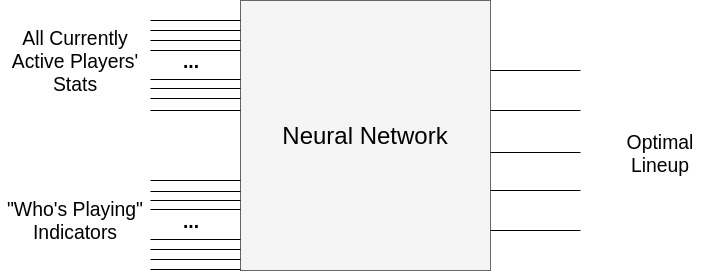
\includegraphics[width=0.75\textwidth]{figures/first_iteration}
    \caption{First design iteration}
    \label{fig:first_iteration}
\end{figure}
 

After discussing this design within our group, and with our supervisor, we realized it had some limitations. First, this system would only use data from active players. This was not taking advantage of the many decades of basketball data that we had access to. Second, it would also likely require a massive amount of data to be able to learn properly. This is because, generally, the amount of data required to learn adequately is correlated with the amount of inputs and complexity of inputs. Third, there would be many unused inputs each time the net is used. Since there are usually only about four NBA games each night, there are only about 80 players active on a single night. There are about 500 total active players, which means that there would be about 420 "unused" inputs. Although this is not explicitly a problem, it makes it seem like there would be a better way to structure the design. The final limitation of the initial neural network that we thought of was that it would be prone to discover "bad" correlations. 
%WEAK%
Since the net only knows which players are playing, and not on which team, it would be bound to find correlations between players that are not playing against each other. To explain, say that NYK is playing against BOS in one game, and GSW is playing against CLE in another. The neural network may find a relationship between someone on BOS and on GSW, even though they are not playing against each other, and games are independent.
%WEAK%
Taking these limitations into account, we decided to come up with an improved architecture that was more flexible and required less data to train. We decided on a three step process, of which only one of the steps would involve machine learning, to start. The three steps are to calculate the player scores, use them in a NN to find good players, and then use a third system to choose lineups. An overview of this software architecture can be seen in Figure \ref{fig:second_iteration}.
\begin{figure}[ht]
    \centering
    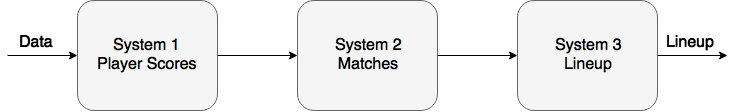
\includegraphics[width=0.85\textwidth]{figures/second_iteration}
    \caption{Redesigned System Architecture}
    \label{fig:second_iteration}
\end{figure}

These three systems will now be looked at in detail.

\paragraph{System 1: Calculating Player Scores}\mbox{}\\
The first step of the design solution is to calculate a score for each player who has played in the NBA. This score is ideally supposed to be a representation of how good the player is, "in a vacuum". That is to say, how well a player will perform if we ignore the match-specific variables like who is on his team, or who he is playing against. Getting a score that represents this is not an exact science. We were initially going to use player rankings given by experts, but could not find historical data for this. Thus, we knew we had to come up with a system of our own to generate these scores. Since we wanted to spend more time focusing on the second system (NN), we decided to initially use a simple equation here based on the player's season statistics, as opposed to something like a neural network. The first equation we decided to use was actually the equation for getting fantasy basketball scores for season fantasy basketball. We postulate that there is a clear correlation between the amount of fantasy points a player would get, and how good of a player they are. Although this is a simplification, it is a good starting point, and due to the modularity of our design, we can always improve it or change it, as long as the inputs and outputs stay the same. 
\begin{figure}[ht]
    \centering
    \includegraphics[width=0.5\textwidth]{figures/player_scores}
    \caption{Player scores system}
    \label{fig:player_scores}
\end{figure}

\paragraph{System 2: Matches Neural Network}\mbox{}\\
The scores for every player, obtained in the first step, are then used as inputs for the matches neural network, the portion of the implementation side of the project that has seen the most development in the first half of the project timeline. The matches neural net puts two teams of players, each represented by a score, "against each other". That is to say, the first ten inputs are used for Team A's players, and the next ten are used for Team B's players.  The output of the net is then a "fantasy game score" for each player that should be higher for players who would get higher fantasy scores. The idea behind this net is that, since all basketball matches follow the same rules, with the only (or at least most impactful) variable being who is playing on each team, we can train this net on every match that has happened in the past 50 years, and still use it on matches today. This net has a minimal amount of inputs, none of which will be unused. This means it needs less data to train successfully. This design can be seen in Figure \ref{fig:neural_network_full}.

\begin{figure}[ht]
    \centering
    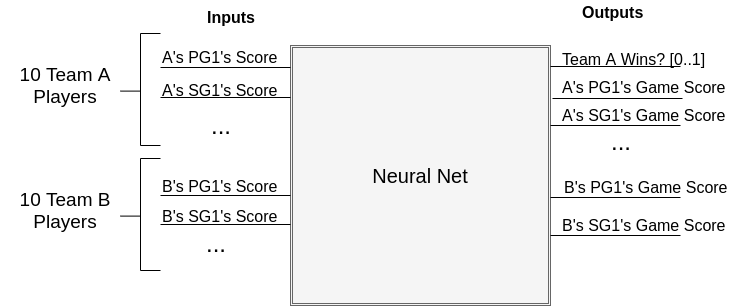
\includegraphics[width=0.6\textwidth]{figures/neural_network_full}
    \caption{Desired complete matches neural network}
    \label{fig:neural_network_full}
\end{figure}

To minimize the debugging phase of this NN, we decided to start with a simple version, and then iterate towards the final version. The more simplified version (the first prototype) output which team would win, instead of the players' game scores. This neural net was thus not applicable for fantasy basketball, but was used instead to become familiar with TensorFlow and best practices. In building this early prototype, we decided to start with a further simplification, namely to only have four inputs: the average player scores and their distribution for each team. Thus, the diagram in Figure \ref{fig:neural_network_full} was simplified to the one seen in Figure \ref{fig:neural_network_averages}.

\begin{figure}[ht]
    \centering
    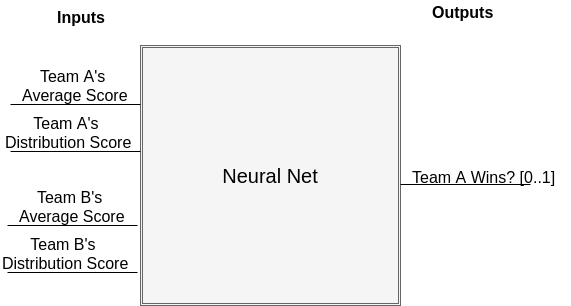
\includegraphics[width=0.4\textwidth]{figures/neural_network_averages}
    \caption{Matches neural network with averaged player scores}
    \label{fig:neural_network_averages}
\end{figure}

The justification behind the inputs and outputs is that the average scores of the players on each team should help to determine which team will win or lose. We found that this neural network was better than random chance at predicting which team would win, with around a 63\% success rate (see the Results subsection for more detail).

We then undid this "averages" simplification, and reverted to having separate inputs for each player. However, since teams do not always play ten players, we used seven instead. We ordered the inputs for each team by the score, so that the first input corresponded to the player on Team A with the highest score. We felt that having ordered scores would help the net learn better, as it would likely learn to put a heavier weight on the higher scores (better players have more impact). This was found to be true in a couple of tests where we used randomized inputs, which were found to be less successful. Using ordered player scores, we had a success rate of around 64\%. The diagram for this net can be seen in Figure \ref{fig:neural_network_ordered}.

\begin{figure}[ht]
    \centering
    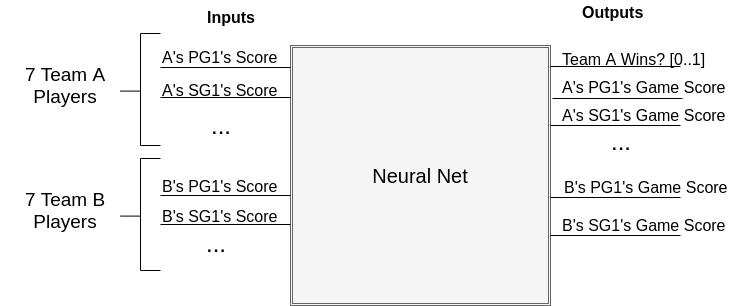
\includegraphics[width=0.6\textwidth]{figures/neural_network_ordered}
    \caption{Matches neural network with ordered player scores}
    \label{fig:neural_network_ordered}
\end{figure}

We decided to iterate towards our final goal once more, and did so by ordering the players on each team by their basketball position. The basketball positions given by our source are guard (G), forward (F), and center (C). As not each team plays the same amount of players in each position, we had to determine what a representative combination of the above positions would look like. This analysis will be discussed in the Data Results section, below. Ultimately, we decided that a representative set for which we had data would be one center (first input), two guards (second and third inputs), and two forwards (fourth and fifth inputs). This net was the same as the initial plan in Figure \ref{fig:neural_network_full}, except with the single winning output rather than the player game scores.

The final aspect of the neural network that we changed in hopes to see better results was the structure of the output. Instead of using a "digital" output, where the game was either won (1) or lost (0), we decided to use an "analog" output. In this case, winning a game by a high amount of points would be close to an output of 1, and losing by a high amount would be close to an output of -1, but values in between are also possible. We felt that this made the most sense, since we felt that our network should be trained on the point difference between teams to yield more confident wins and losses. To decide how to map the point difference in a game to [0,1], we first discussed with people familiar with the sport what the difference is between a team winning a game by 20 points versus winning by 2 points. We came to the conclusion that, generally speaking, if a team wins by 15 points, they won rather handily, and anything closer to 0 points could have gone either way. With this in mind, we decided to use a scaled arctangent function, such that, around a difference of 15 points, the output is around a value of 1, and that it tapers off after this. The equation used for this can be seen in (Eq 1). The shape of this mapping can be seen in Figure \ref{fig:arctanShape}. One can see that this function can output a value greater than 1 (at a point difference of about 25 points), but this was not a great concern. Even with a point difference of 50 points, which is unlikely, the output is only ~1.27.

\begin{equation}
Output = arctan(pointDifference/15)
\end{equation}

\begin{figure}[ht]
    \centering
    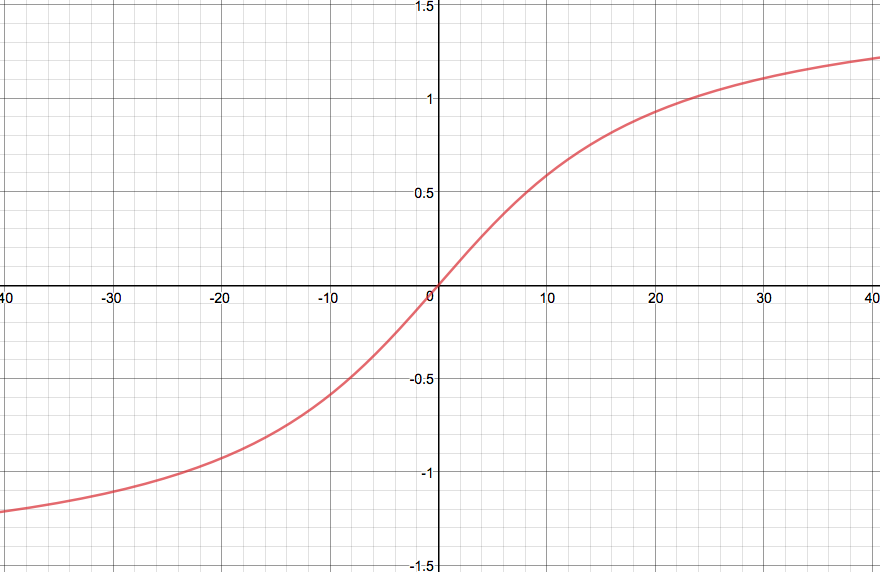
\includegraphics[width=0.6\textwidth]{figures/arctanShape}
    \caption{Shape of modified arctangent used for mapping point difference to output}
    \label{fig:arctanShape}
\end{figure}


The results of the final version of this prototype can be seen in the results section. This is not the version that will be used for our final project; the next step will be to change the outputs from which team wins to player game scores. This will be discussed in the Future Plans section.

\paragraph{System 3: Choosing Lineups}\mbox{}\\
The choosing lineups system will be the system that actually outputs lineups to enter into the fantasy competition. Although this system has not been built yet, the inputs and outputs have been designed. It will take in the properties of the fantasy competition, such as the budget, the positions needed, and the teams playing, as well as all of the players' game scores from system 2. Using these inputs, it will output a set of lineups that meet all the necessary competition constraints (e.g. below the budget), that maximize the overall score.

\subsection{Results}
There are two types of results that will be given in this report. The first are those related to how much data was scraped from our source, or generated, and the second is related to the success rate of the neural network.

\subsubsection{Data Results}
We managed to scrape, collect, and otherwise compute a significant amount of data to be stored in our database. We were able to gather all data for every basketball game since 1979. We have data for 42000 matches, 10000 player-seasons (unique players for a specific season), 2000 players, and 36 teams, including some that are no longer active. For each match, there are about 15 players with statistics for that match. This is entered in our "player matches" table, and we currently have data in this table for about 25\% of matches. This corresponds to 250,000 entries, and yields about 13000 inputs for our neural net. However, the different architectures which have been presented all impose different constraints on the inputs themselves. For example, the neural network with ordered player scores shown in Figure \ref{fig:neural_network_ordered} requires the match input to have both teams with at least the minimum number of  players (7 in this instance). The neural net with players ordered by position has even more constraints. Not only does it require a minimum number of players per team, but also it needs a minimum number of players per \textit{position}. When performing an analysis on the different player positions per lineup, we found significant variation between teams. This was even further complicated as some players played multiple positions, denoted by two positions separated by a hyphen. For example, the position "F-G" meant that the player could either play a forward or a guard. We found 21 possible combinations of these positions that teams could play. As an example, playing "C, G, G, F, F, C-F" could be a single combination, whereas "F-G, C, C-F, F, F, G, G" could be another. We found that none of the possible 21 combinations had enough data to train our neural network on. Even our initially designed input format of requiring two guards, one center, and two forwards per team (meaning only five inputs per team) caused roughly 21\% of inputs to be discarded, simply because these inputs did not meet the criteria of having these specific numbers of players in each positions.

To avoid losing significant amounts of input data due to constraints, we simplified our input scheme by combining the multi-position players with the single-position players. Our methods of combining these players is shown in Figure \ref{fig:distributionAfterCombination} below. In using this scheme, we were able to reduce the amount of lost data to a mere 11\%.

\begin{figure}[ht]
    \centering
    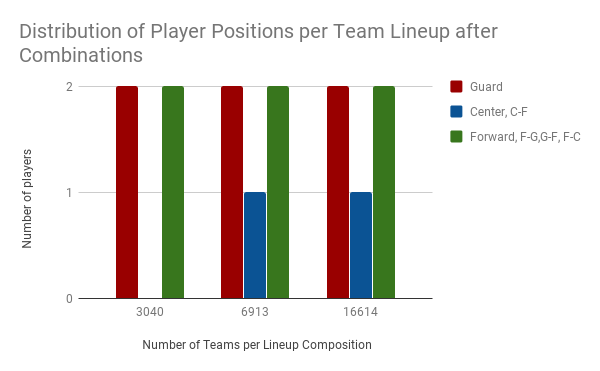
\includegraphics[width=0.75\textwidth]{figures/distributionAfterCombination}
    \caption{Team Compositions by Player Positions After Combinations}
    \label{fig:distributionAfterCombination}
\end{figure}

\subsubsection{Implementation Results}
As mentioned in the description of the neural network in the implementation section, we went through a few different architectures. Although the final architecture will be one that takes in the player scores in order of position, and outputs game scores for each of the players, this has not been built yet. However, for the first three architectures, we have collected some results. The main result collected is the win-loss prediction success rate, as related the amount of data used and the architecture of the inputs and outputs. All other ML parameters, such as learning rate and number of hidden nodes, remained unchanged. The neural network has only one hidden layer for simplicity. Furthermore, all accuracy results were obtained by using 70\% of the input data to train the network, and 30\% to test.\\

The first architecture that we tested was the one shown in Figure \ref{fig:neural_network_averages}. Because the input of this neural network consisted solely of averages and variances for each team, we were able to use all of our data (100\%) to train and test the network. The highest testing accuracy was around 63\% for this architecture, as can be seen in Figure \ref{fig:accuracyAveragedInputs}, which shows the success of the neural net versus the epoch number, or the number of times the entire data set has been passed through the neural network. As the epoch increases, the accuracy should converge. It does not always converge asymptotically, and in these cases, the method for determining when a network has reached its true accuracy rate is when the training accuracy separates from, and surpasses, the testing accuracy. In these cases, the neural network is overfitting the training data, and achieving higher accuracy rates, but it is not representative of a real relationship.

\begin{figure}[ht]
    \centering
    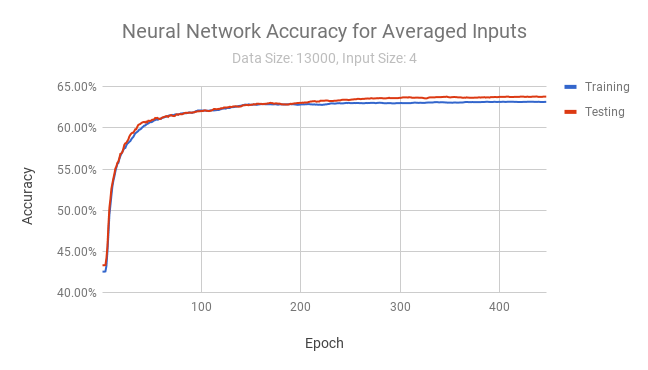
\includegraphics[width=0.6\textwidth, frame]{figures/accuracyAveragedInputs}
    \caption{Accuracy of network for averaged player scores inputs}
    \label{fig:accuracyAveragedInputs}
\end{figure}


After testing the averages, we tested the version of the neural network where the inputs were the actual player scores on each team, ordered from highest to lowest (previously shown in Figure \ref{fig:neural_network_ordered}). We tested this with two different configurations; first by taking the top five players on each team, and then the top 7 players on each team. The accuracy for both of these scenarios can be seen in Figure \ref{fig:accuracy5Scores} and Figure \ref{fig:accuracy7Scores}. One can see that having more scores as inputs does increase the accuracy, and by a significant margin in this case. However, it is also worth noting that this increase is also tied to the increase in data between the two cases (9000 vs. 10000). When both are set to use the same amount of data, the improvement is less significant.

\begin{figure}[ht]
    \centering
    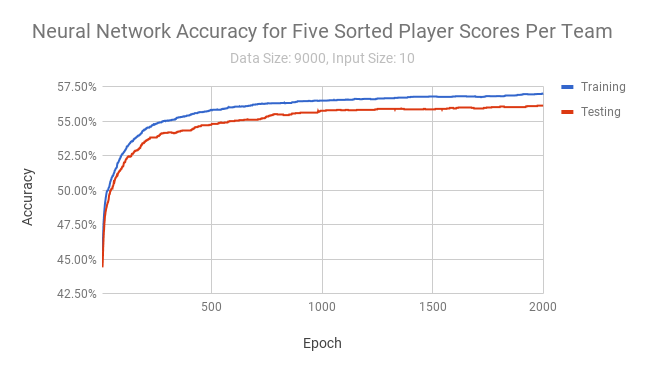
\includegraphics[width=0.6\textwidth, frame]{figures/accuracy5Scores}
    \caption{Accuracy of network for 5 player scores inputs per team}
    \label{fig:accuracy5Scores}
\end{figure}

\begin{figure}[ht]
    \centering
    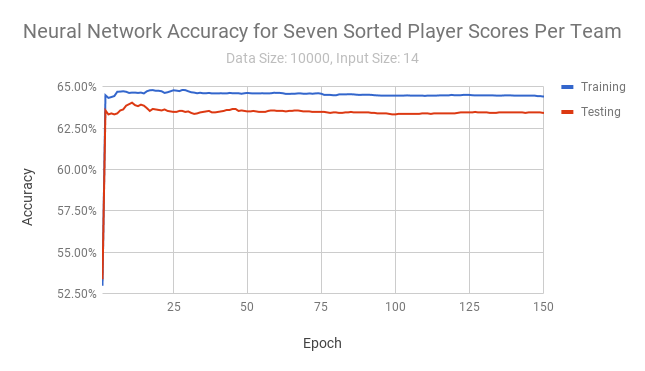
\includegraphics[width=0.6\textwidth, frame]{figures/accuracy7Scores}
    \caption{Accuracy of network for 7 player scores inputs per team}
    \label{fig:accuracy7Scores}
\end{figure}

As mentioned earlier, in an attempt to further increase the accuracy, we switched to having 5 inputs (or players) on each team, but ordered by their position. To reiterate, we grabbed the highest two guard (G) scores, the highest two forward (F) scores, and the highest center (C) score, and used these as the inputs per team, in that order. The accuracy for this network can be seen in Figure \ref{fig:accuracyPositions}. One can see that this did not increase the accuracy of the net by a significant amount. However, we believe that this is the best structuring of inputs to use, as it allows the network to learn that the first position is always tied to a guard, which may have more or less impact than other positions (as opposed to using ordered scores). We believe that the reason we did not see a significant increase in the accuracy is because, with only 5 players per team, and sorted by position, we often cut out some top players. Ideally, we would be able to select a more representative position set (as opposed to G, G, F, F, C) that would allow us to use more inputs (players) for the net.

\begin{figure}[ht]
    \centering
    \includegraphics[width=0.6\textwidth, frame]{figures/accuracyPositions}
    \caption{Accuracy of network for positionally ordered score inputs}
    \label{fig:accuracyPositions}
\end{figure}

In addition to changing the structure of the inputs to try to obtain higher accuracy rates for our neural network, we also worked on changing some of the other parameters. First, we tried to check the impact of using more or less data. We found that the impact could be quite significant, and that, usually, more data led to a higher accuracy rate. An extreme version of this can be seen in Figure \ref{fig:accuracyData}. However, there was one case in which only using the most recent two thousand games actually yielded a higher accuracy. This could just be that the sample size was too small to gather any meaningful conclusions from, but it could also imply that using data from ten years ago for current games may be a bad idea, as basketball may have changed too much. This is something that will be explored when we build the next and final neural net architecture.

\begin{figure}[ht]
    \centering
    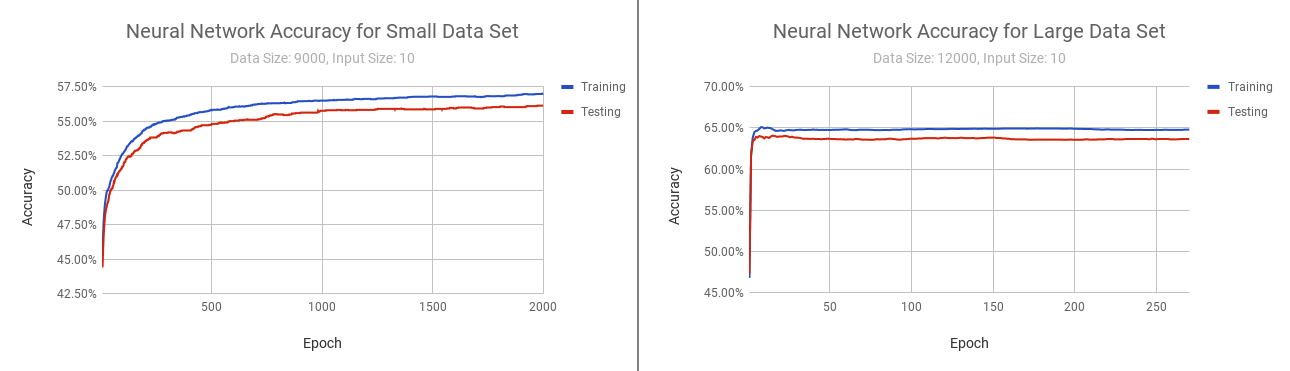
\includegraphics[width=1\textwidth, frame]{figures/accuracyData}
    \caption{Accuracy of neural network vs. amount of data used}
    \label{fig:accuracyData}
\end{figure}


The next parameters that we wanted to alter were those related to the neural net's properties, namely the number of hidden layers, hidden nodes, and learning rate. We changed these by hand and saw changes to the net's accuracy, and were able to manipulate these to make minor improvements. We did not optimize these parameters thoroughly, as it was out of the scope of this semester, and since this neural net was only a prototype. As will be discussed in the Future Plans section, we did find a way to optimize these parameters, namely n-fold cross validation. 
